\section{Definitions and nomenclature}

\subsection{Systems and Stability}
In order to define stable learning algorithms, it is imperal to firstly define, first-order systems and stability, which is taken from \cite{khalilNonlinearSystems1996}.

\begin{definition}[First-Order System]
    A continuous-time first-order system is defined by the following map
    \begin{equation}
        f:\mathbb{R}\times\mathbb{R}\rightarrow \mathbb{R}, (x(t),u(t)) \mapsto \dot x(t) = f(x(t),u(t)).
        \label{def:eq-system}
    \end{equation}

    Additionally, if $u(t)$ is a function of $x$, the system is autonomous, with closed-loop dynamics $f(x(t)$). The trajectory of the system is defined by the evolution of $x(t)$. Furthermore, the system has an equilibrium point at $f(x(t))=0$.
    \label{def:system}
\end{definition}

\begin{definition}[Stability]
    Consider the equilibrium point $x=0$ of \eqref{def:eq-system}. Then the system is... 
    \begin{itemize}
        \item \textit{stable}, if for each $\epsilon>0$, there is a $\delta>0$, sich that
            $$||x(0)||<\delta \Rightarrow ||x(t)||<\epsilon, \quad \forall t \geq 0$$ 
        \item \textit{unstable}, if not stable, and
        \item \textit{asymptotically stable} if it is stable and $\delta$ can be chosen such that
            $$||x(0)||<\delta \Rightarrow \lim_{t\rightarrow\infty} x(t)=0 $$
    \end{itemize} 
\end{definition}
From here henceworth, the dependency of the dynamics on time is considered to be implicit and will be neglected in the notation.


\begin{definition}[Lyapunov function]
    A Lyapunov function is a continuous function $V: \mathbb{R}^n\rightarrow\mathbb{R}$ with the following properties:
    \begin{enumerate}
        \item[(a)] positive definitness: $V(x)>0, \quad \forall x\in\mathbb{R}^n\setminus\{0\}$ and $V(0)=0$,
        \item[(b)] decrease condition: $\dot V(x)\leq0, \quad \forall x\in\mathbb{R}$.
    \end{enumerate}
\end{definition}

\begin{definition}[Stability in the sense of Lyapunov]
    If there exists a continuous function $V: \mathbb{R}^n \rightarrow \mathbb{R}$ such that
     \begin{enumerate}
       \item[(a)] $V(x)$ is positive definite, and
       \item[(b)] $\dot{V}(x)\leq-l(x)$, for some positive semidefinite function $l(x)$,
     \end{enumerate}
    then the system is considered to be stable. Additionally, if $l(x)$ is positive definite, then the system is asymptotically stable.
     \label{def:lyapunov-stability}
\end{definition}

The ultimate goal of this research is to develop stable update laws for neural network (NN) controllers. Hence, the designed control law will be considered as a NN. Hence, NNs are defined as follows throughout this work.

\begin{definition}[Neural network]
    A neural network (NN) $\phi:\mathbb{R}^n\rightarrow \mathbb{R}^p$ is defined as:
   
     \begin{equation}
      \begin{aligned}
        \phi (x) & = (L_1 \circ \varphi_1 \dots \circ L_{H-1} \circ \varphi_{H-1} \circ L_{H} \circ \varphi_H)(x)\\
        L_i(x) &= \theta_i x + b_i \quad \forall i\in\{1,..., H\},
      \end{aligned}
    \end{equation}
  
     where $\varphi_i(\cdot)$ are called  activation functions, $\theta_i$ and $b_i$ are the weight matrix and bias of layer $i$, respectively.
\end{definition}
Whenever, a bias is not mentioned it is assumed to be zero.

NNs usually make use of nonlinear activation functions, which enable them to approximate nonlinear functions. Typically, functions such as the hyperbolic tangent, sigmoid, or ReLU are used in machine learning. This work will utilize an actiavtion function that is designed to model a smooth saturation function, as used in \cite{wahby, thanhNonlinearPIDControl2006} and defined in \eqref{eq:sigmoid}. Note, that it activation function saturates at $\pm \frac{2}{a}$.

\begin{equation}
    \sigma (x) = \frac{2(1-e^{-ax})}{a(1+e^{-ax})}
    \label{eq:sigmoid}
\end{equation}

\subsection{Model Reference Adaptive Control}

\begin{figure}[ht]
    \centering
    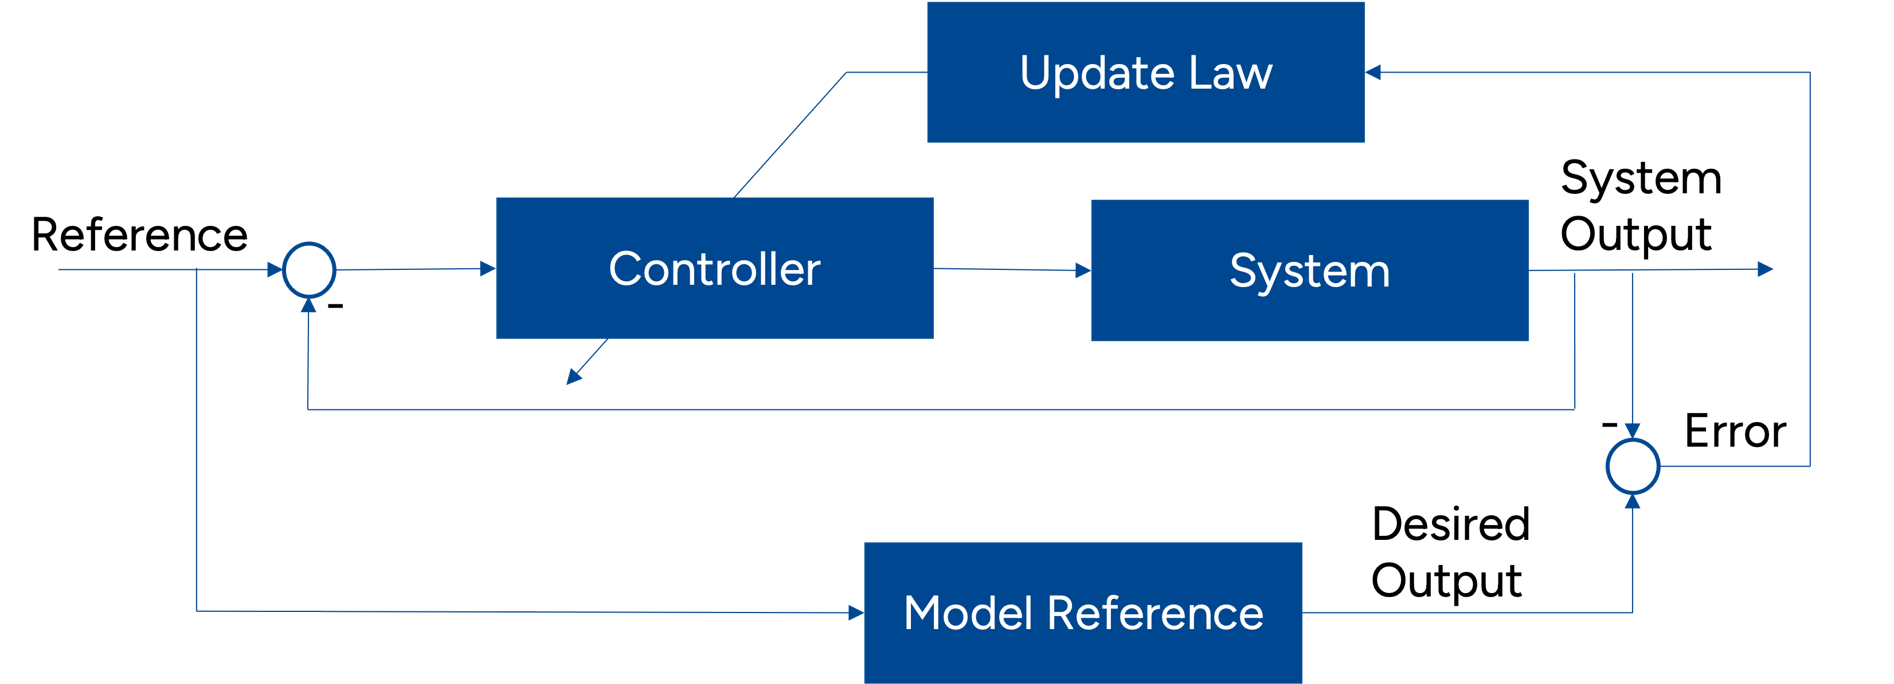
\includegraphics[width=0.8\linewidth]{images/MRAC_Blockdiagram.png}
    \caption{MRAC for first-oder systems controlled by simple NNCs}
    \label{fig:nonlinear-NNC-MRAC}
\end{figure}

\section{Nonlinear Model Reference Adaptive Control (NMRAC)}
\label{sec:MRAC-Nonlinear-SISO}


One of the goal of this work is to analyse stability properties of nonlinear NNCs. To this end, we propose stable update scheme. We commence by looking at the simpler case of a first-order system. More, specifically, we define a problem, where we show that the even in the nonlinear case, we are able to learn a parameter with an algorithm that is based on the logic of a linear MRAC. We call this nonlinear Model Reference Adaptive Control (NMRAC).

We desire to control a system of the form, as described in equation \eqref{eq:first-order-system}, where $\phi: \mathbb{R}\rightarrow\mathbb{R}$ is a nonlinear function, $e_x=x_r - x$,and $\theta$ is the parameter we aim to learn. Here, we would like to point that $\theta$ can be seen as a weight, and $\phi$ the activation function of a NN of the form of a sigmoidial saturation function, as described in equation \eqref{eq:sigmoid}.

\begin{equation}
    \dot x = -ax + b\phi(\theta e_x)
    \label{eq:first-order-system}
\end{equation}

Next, we define a stable reference model, as defined in equation \eqref{eq:first-order-ref}, where $e_m=x_r - x_m$, and $a_m>0$. Note, that we want $\phi_m$ to be of the same form as $\phi$.

\begin{equation}
    \dot x_m = -a_mx_m + b_m\phi_m(\theta_m e_m)
    \label{eq:first-order-ref}
\end{equation}

Since we aim for the system to follow the reference model, we define the error dynamics as in equation \eqref{eq:error-dynamics-nonlinear}. Note, that from this definition it follows that $e=e_x-e_m$. We will use this alternative definition later for the stability analysis of the update law.

\begin{equation}
    e=x_m-x
    \label{eq:error-dynamics-nonlinear}
\end{equation}

Following the error dynamics, we define the Lyapunov candidate to be defined as in equation \eqref{eq:nonlinear-lyapunov-candidate}. The factor $c>0$, is used to accelerate or decelerate the learning process. The norm of the error captures the distance between the internal states of the reference model and the system, and the term $||\alpha||_2^2$ captures the distance between the NNC and the desired NNC, which can be seen as the difference in dynamics between the controlled system and the model reference. Note, that both $e$ and $\alpha$ should be $0$, when our system follows the reference model and the desired parameters are learned. Futhermore, this property renders our Lyapunov candidate to be positive definite.

\begin{equation}
    V(e, \alpha) =||e||_2^2 + ||c \alpha||_2^2
    \label{eq:nonlinear-lyapunov-candidate}
\end{equation}

To ensure that the controlled system is stable, we require the time derivative of the Lyapunov function to be negative. Therefore, we analyze the behavior of the resulting time derivative of the Lyapunov function. The resulting equation is defined in \eqref{eq:nonlinear-lyapunov-derivative}.

\begin{equation}
    \begin{aligned}
    \dot V(e, \alpha) = & 2e\dot e + 2\alpha \dot \alpha c
    \end{aligned}
    \label{eq:nonlinear-lyapunov-derivative}
\end{equation}

We now construct the time derivative of the error dynamics, which is defined by equation \eqref{eq:nonlinear-error-time-derivative}. We extend the equation by $\pm (a_mx b_m \phi_m(\theta_m e_x))$, to construct the term $\alpha$, which is now dependent on $e_x$, and $\theta$. We are then left with two other terms, namely, $-a_me$, and $\gamma_m(e_m, e_x)$.

\begin{equation}
    \begin{aligned}
    \dot e 
= & \dot x_m - \dot x \\ 
= & -a_mx_m + b_m\phi_m(\theta_me_m) - (-ax + b\phi(\theta e_x)) \\
    & \pm (a_mx + b_m \phi_m(\theta_m e_x)) \\
    = & -a_m \underbrace{(x_m-x)}_{=e} \\ 
    & + \underbrace{(a-a_m)x+b_m\phi_m(\theta_me_x) - b\phi(\theta e_x)}_{=\alpha(e_x, \theta)} \\ 
    & + \underbrace{b_m(\phi_m(\theta_m e_m)-\phi_m(\theta_m e_x))}_{=\gamma_m(e_m,e_x)}
    \end{aligned}
    \label{eq:nonlinear-error-time-derivative}
\end{equation}

\begin{equation}
    \begin{aligned}
    \dot V(e, \alpha) 
    = & 2e(-a_me + \alpha(e_x, \theta) + \gamma_m(e_m, e_x)) + 2\alpha c \dot \alpha(e_x, \theta)\\
    = & -2a_me^2 \\ 
    & + 2e\gamma_m(e_m, e_x) 
    \\ 
    & + 2\alpha(e_x, \theta)(e + c \dot \alpha(e_x, \theta))
    \end{aligned}
    \label{eq:nonlinear-lyapunov-derivative2}
\end{equation}

By substituting equation \eqref{eq:nonlinear-error-time-derivative} into equation \eqref{eq:nonlinear-lyapunov-derivative}, we get equation \eqref{eq:nonlinear-lyapunov-derivative2}. 

Note, that the first term $-2a_me^2$ is always negative, since $a_m>0$, and $e^2 > 0$. The second term will always be negative, due to the property of $e=e_x-e_m$. It follows that if $e<0 \Rightarrow \gamma_m(e_m, e_x)>0$, which implies that the second term is negative, and if $e>0 \Rightarrow \gamma_m(e_m, e_x)<0$, which again implies that the second term is negative. Hence, the second term reamins negative.

Since, we can already ensure that the first two terms of equation \eqref{eq:nonlinear-lyapunov-derivative2} are negative, it remains to show that the last term is always negative or equal to zero at all times. Since $\theta$ is dependent on time, this implies $\dot \alpha(e_x, \theta)$ will have a term that includes $\dot \theta$. Therefore, we choose  $\dot \theta$, such that the third term in equation \eqref{eq:nonlinear-lyapunov-derivative2} is nullified. Note, that due to the way we construct the update law, stability is guaranteed, since the Lyapunov function is positive definite and simultaneously the decrease condition is satisfied.

% \begin{equation}
%     \begin{aligned}
%         0 = & 2\alpha(e_x, \theta)(e +  \dot \alpha(e_x, \theta)) \\
%         \Leftrightarrow 0 = & e +  c \dot \alpha(e_x, \theta) \\
%         \Leftrightarrow 0 = & e + c \left[ (a-a_m)\dot x +b_m \frac{d\phi_m(\theta_me_x)}{dt} - b \frac{d\phi(\theta e_x)}{d t} \right]\\
%         \Leftrightarrow 0 = & \frac{1}{c}e + (a-a_m)\dot x +b_m \frac{\partial \phi_m(\tilde x)}{\partial \tilde x}\vert_{\tilde \theta e_x = \theta e_x}\theta_m \dot e_x - b \frac{d\phi(\tilde x)}{\partial \tilde x}\vert_{\tilde x = \theta e_x}(e_x \dot\theta + \theta \dot e_x)
%     \end{aligned}
% \end{equation}

\begin{equation}
    \begin{aligned}
        0 = & 2\alpha(e_x, \theta)(e +  \dot \alpha(e_x, \theta))
    \end{aligned}
\end{equation}

\begin{equation}
    \begin{aligned}
     \dot \theta & = \frac{1}{e_x b \frac{\partial \phi(\tilde x)}{\partial \tilde x}\vert_{\tilde x=\theta e_x}}\\ 
     & (  \frac{1}{c} e + (a-a_m)\dot x + b_m\frac{\partial \phi_m(\tilde x)}{\partial \tilde x}\vert_{\tilde x=\theta_me_x}\theta_m \dot e_x) \\ 
    & - \frac{\theta}{e_x}\dot e_x
    \end{aligned}
    \label{eq:nonlinear-update-law}
\end{equation}

When taking a closer look at the update rule in equation \eqref{eq:nonlinear-update-law}, it follows that we require to implement an update hold, when $e_x=0$. This is reasonable, since whenever the state of our reference system is equal to the reference signal, we will not be able to extract information on how to change the weights in order for our system to converge towards the reference signal. In practice this means that we implement a threshold $\varepsilon$, where we do not update the weights.